%======================================================================
\chapter{Experimental Results}
%======================================================================
\label{ch:results}

%\begin{sidewaystable*}[htbp]
%\centering
%\caption{Ranking effectiveness on Robust04, Core17 and Core18}
%\begin{center}
%\resizebox{\columnwidth}{!}{
%\begin{tabular}{lcc ccc ccc ccc}
%\toprule
% & \multicolumn{3}{c}{\textbf{Robust04}} & \multicolumn{3}{c}{\textbf{Core17}} & \multicolumn{3}{c}{\textbf{Core18}} \\
% \cmidrule(lr){2-4}  \cmidrule(lr){5-7}  \cmidrule(lr){8-10}
%{\bf Model} & {\bf MAP} & {\bf P@20} & {\bf NDCG@20}   & {\bf MAP}  & {\bf P@20} & {\bf NDCG@20} & {\bf MAP} & {\bf P@20} & {\bf NDCG@20}  \\
%
%\toprule
%
%\textbf{BM25+RM3} & 0.2903 & 0.3821 & 0.4407 & 0.2823 & 0.5500 & 0.4467 & 0.3135 & 0.4700 & 0.4604 \\
%
%\midrule
%
%\textbf{1S: $ \textrm{BERT}(\textrm{MB}) $} & 0.3408$^{\dagger}$ & 0.4335$^{\dagger}$ & 0.4900$^{\dagger}$ & 0.3091$^{\dagger}$ & 0.5620 & 0.4628 & 0.3393$^{\dagger}$ & 0.4930 & 0.4848$^{\dagger}$  \\
%\textbf{2S: $ \textrm{BERT}(\textrm{MB}) $} & 0.3435$^{\dagger}$ & 0.4386$^{\dagger}$ & 0.4964$^{\dagger}$ & 0.3137$^{\dagger}$ & 0.5770 & 0.4781 & 0.3421$^{\dagger}$ & 0.4910 & 0.4857$^{\dagger}$  \\
%\textbf{3S: $ \textrm{BERT}(\textrm{MB}) $} & 0.3434$^{\dagger}$ & 0.4422$^{\dagger}$ & 0.4998$^{\dagger}$ & 0.3154$^{\dagger}$ & 0.5880 & 0.4852$^{\dagger}$ & 0.3419$^{\dagger}$ & 0.4950$^{\dagger}$ & 0.4878$^{\dagger}$ \\
%
%\midrule
%
%\textbf{1S: $ \textrm{BERT}(\textrm{CAR}) $} & 0.3025$^{\dagger}$ & 0.3970$^{\dagger}$ & 0.4509 & 0.2814$^{\dagger}$ & 0.5500 & 0.4470 & 0.3120 & 0.4680 & 0.4586 \\
%\textbf{2S: $ \textrm{BERT}(\textrm{CAR}) $} & 0.3025$^{\dagger}$ & 0.3970$^{\dagger}$ & 0.4509 & 0.2814$^{\dagger}$ & 0.5500 & 0.4470 & 0.3116 & 0.4670 & 0.4585 \\
%\textbf{3S: $ \textrm{BERT}(\textrm{CAR}) $} & 0.3025$^{\dagger}$ & 0.3970$^{\dagger}$ & 0.4509 &  0.2814$^{\dagger}$ & 0.5500 & 0.4470 & 0.3113 & 0.4670 & 0.4584 \\
%
%\midrule
%
%\textbf{1S: $ \textrm{BERT}(\textrm{MS MARCO}) $} & 0.3028$^{\dagger}$ & 0.3964$^{\dagger}$ & 0.4512 & 0.2817$^{\dagger}$ & 0.5500 & 0.4468 & 0.3121 & 0.4670 & 0.4594 \\
%\textbf{2S: $ \textrm{BERT}(\textrm{MS MARCO}) $} & 0.3028$^{\dagger}$ & 0.3964$^{\dagger}$ & 0.4512 & 0.2817$^{\dagger}$ & 0.5500 & 0.4468 & 0.3121 & 0.4670 & 0.4594 \\
%\textbf{3S: $ \textrm{BERT}(\textrm{MS MARCO}) $} & 0.3028$^{\dagger}$ & 0.3964$^{\dagger}$ & 0.4512 & 0.2817$^{\dagger}$ & 0.5500 & 0.4468 & 0.3121 & 0.4670 & 0.4594 \\
%
%\midrule
%
%\textbf{1S: $ \textrm{BERT}(\textrm{CAR}\rightarrow\textrm{MB}) $} & 0.3476$^{\dagger}$ & 0.4380$^{\dagger}$ & 0.4988$^{\dagger}$ & 0.3103$^{\dagger}$ & 0.5830 & 0.4758 & 0.3385$^{\dagger}$ & 0.4860 & 0.4785 \\
%\textbf{2S: $ \textrm{BERT}(\textrm{CAR}\rightarrow\textrm{MB}) $} & 0.3470$^{\dagger}$ & 0.4400$^{\dagger}$ & 0.5015$^{\dagger}$ & 0.3140$^{\dagger}$ & 0.5830 & 0.4817$^{\dagger}$ & 0.3386$^{\dagger}$ & 0.4810 & 0.4755 \\
%\textbf{3S: $ \textrm{BERT}(\textrm{CAR}\rightarrow\textrm{MB}) $} & 0.3466$^{\dagger}$ & 0.4398$^{\dagger}$ & 0.5014$^{\dagger}$ & 0.3143$^{\dagger}$ & 0.5830 & 0.4807 & 0.3382$^{\dagger}$ & 0.4830 & 0.4731 \\
%
%\midrule
%
%\textbf{1S: $ \textrm{BERT}(\textrm{MS MARCO}\rightarrow\textrm{MB}) $} & 0.3676$^{\dagger}$ & 0.4610$^{\dagger}$ & 0.5239$^{\dagger}$ & 0.3292$^{\dagger}$ & 0.6080$^{\dagger}$ & 0.5061$^{\dagger}$ & 0.3486$^{\dagger}$ & {\bf 0.4920} & {\bf 0.4953}$^{\dagger}$ \\
%\textbf{2S: $ \textrm{BERT}(\textrm{MS MARCO}\rightarrow\textrm{MB}) $} & {\bf 0.3697}$^{\dagger}$ & 0.4657$^{\dagger}$ & 0.5324$^{\dagger}$ & {\bf 0.3323}$^{\dagger}$ & 0.6170$^{\dagger}$ & {\bf 0.5092}$^{\dagger}$ & 0.3496$^{\dagger}$ & 0.4830 & 0.4899$^{\dagger}$ \\
%\textbf{3S: $ \textrm{BERT}(\textrm{MS MARCO}\rightarrow\textrm{MB}) $} & 0.3691$^{\dagger}$ & {\bf 0.4669}$^{\dagger}$ & {\bf 0.5325}$^{\dagger}$ & 0.3314$^{\dagger}$ & {\bf 0.6200}$^{\dagger}$ & 0.5070$^{\dagger}$ & {\bf 0.3522}$^{\dagger}$ & 0.4850 & 0.4899$^{\dagger}$ \\
%
%\bottomrule
%\end{tabular}
%}
%\label{tab:results}
%\end{center}
%\end{sidewaystable*}

%%%%%

\begin{table*}[b!]
\centering\resizebox{0.7\columnwidth}{!}{
\begin{tabular}{lcc ccc}
\toprule
% & \multicolumn{3}{c}{\textbf{Robust04}} \\
% \cmidrule(lr){2-4}
{\bf Model} & {\bf MAP} & {\bf P@20} & {\bf NDCG@20}  \\
\toprule
\textbf{BM25+RM3} & 0.2903 & 0.3821 & 0.4407 \\
\midrule
\textbf{1S: $ \textrm{BERT}(\textrm{MB}) $} & 0.3408$^{\dagger}$ & 0.4335$^{\dagger}$ & 0.4900$^{\dagger}$  \\
\textbf{2S: $ \textrm{BERT}(\textrm{MB}) $} & 0.3435$^{\dagger}$ & 0.4386$^{\dagger}$ & 0.4964$^{\dagger}$  \\
\textbf{3S: $ \textrm{BERT}(\textrm{MB}) $} & 0.3434$^{\dagger}$ & 0.4422$^{\dagger}$ & 0.4998$^{\dagger}$ \\
\midrule
\textbf{1S: $ \textrm{BERT}(\textrm{CAR}) $} & 0.3025$^{\dagger}$ & 0.3970$^{\dagger}$ & 0.4509 \\
\textbf{2S: $ \textrm{BERT}(\textrm{CAR}) $} & 0.3025$^{\dagger}$ & 0.3970$^{\dagger}$ & 0.4509 \\
\textbf{3S: $ \textrm{BERT}(\textrm{CAR}) $} & 0.3025$^{\dagger}$ & 0.3970$^{\dagger}$ & 0.4509  \\
\midrule
\textbf{1S: $ \textrm{BERT}(\textrm{MS MARCO}) $} & 0.3028$^{\dagger}$ & 0.3964$^{\dagger}$ & 0.4512 \\
\textbf{2S: $ \textrm{BERT}(\textrm{MS MARCO}) $} & 0.3028$^{\dagger}$ & 0.3964$^{\dagger}$ & 0.4512 \\
\textbf{3S: $ \textrm{BERT}(\textrm{MS MARCO}) $} & 0.3028$^{\dagger}$ & 0.3964$^{\dagger}$ & 0.4512 \\
\midrule
\textbf{1S: $ \textrm{BERT}(\textrm{CAR}\rightarrow\textrm{MB}) $} & 0.3476$^{\dagger}$ & 0.4380$^{\dagger}$ & 0.4988$^{\dagger}$ \\
\textbf{2S: $ \textrm{BERT}(\textrm{CAR}\rightarrow\textrm{MB}) $} & 0.3470$^{\dagger}$ & 0.4400$^{\dagger}$ & 0.5015$^{\dagger}$ \\
\textbf{3S: $ \textrm{BERT}(\textrm{CAR}\rightarrow\textrm{MB}) $} & 0.3466$^{\dagger}$ & 0.4398$^{\dagger}$ & 0.5014$^{\dagger}$ \\
\midrule
\textbf{1S: $ \textrm{BERT}(\textrm{MS MARCO}\rightarrow\textrm{MB}) $} & 0.3676$^{\dagger}$ & 0.4610$^{\dagger}$ & 0.5239$^{\dagger}$ \\
\textbf{2S: $ \textrm{BERT}(\textrm{MS MARCO}\rightarrow\textrm{MB}) $} & {\bf 0.3697}$^{\dagger}$ & 0.4657$^{\dagger}$ & 0.5324$^{\dagger}$ \\
\textbf{3S: $ \textrm{BERT}(\textrm{MS MARCO}\rightarrow\textrm{MB}) $} & 0.3691$^{\dagger}$ & {\bf 0.4669}$^{\dagger}$ & {\bf 0.5325}$^{\dagger}$ \\
\bottomrule
\end{tabular}
}
\caption{Ranking effectiveness on Robust04.}
\label{tab:results-robust04}
\end{table*}

\begin{table*}
\centering\resizebox{0.7\columnwidth}{!}{
\begin{tabular}{lcc ccc}
\toprule
% & \multicolumn{3}{c}{\textbf{Robust04}} \\
% \cmidrule(lr){2-4}
{\bf Model} & {\bf MAP} & {\bf P@20} & {\bf NDCG@20}  \\
\toprule
\textbf{BM25+RM3} & 0.2823 & 0.5500 & 0.4467 \\
\midrule
\textbf{1S: $ \textrm{BERT}(\textrm{MB}) $} & 0.3091$^{\dagger}$ & 0.5620 & 0.4628  \\
\textbf{2S: $ \textrm{BERT}(\textrm{MB}) $} & 0.3137$^{\dagger}$ & 0.5770 & 0.4781 \\
\textbf{3S: $ \textrm{BERT}(\textrm{MB}) $} & 0.3154$^{\dagger}$ & 0.5880 & 0.4852$^{\dagger}$ \\
\midrule
\textbf{1S: $ \textrm{BERT}(\textrm{CAR}) $} & 0.2814$^{\dagger}$ & 0.5500 & 0.4470 \\
\textbf{2S: $ \textrm{BERT}(\textrm{CAR}) $} & 0.2814$^{\dagger}$ & 0.5500 & 0.4470 \\
\textbf{3S: $ \textrm{BERT}(\textrm{CAR}) $} & 0.2814$^{\dagger}$ & 0.5500 & 0.4470 \\
\midrule
\textbf{1S: $ \textrm{BERT}(\textrm{MS MARCO}) $} & 0.2817$^{\dagger}$ & 0.5500 & 0.4468 \\
\textbf{2S: $ \textrm{BERT}(\textrm{MS MARCO}) $} & 0.2817$^{\dagger}$ & 0.5500 & 0.4468 \\
\textbf{3S: $ \textrm{BERT}(\textrm{MS MARCO}) $} & 0.2817$^{\dagger}$ & 0.5500 & 0.4468 \\
\midrule
\textbf{1S: $ \textrm{BERT}(\textrm{CAR}\rightarrow\textrm{MB}) $} & 0.3103$^{\dagger}$ & 0.5830 & 0.4758  \\
\textbf{2S: $ \textrm{BERT}(\textrm{CAR}\rightarrow\textrm{MB}) $} & 0.3140$^{\dagger}$ & 0.5830 & 0.4817$^{\dagger}$ \\
\textbf{3S: $ \textrm{BERT}(\textrm{CAR}\rightarrow\textrm{MB}) $} & 0.3143$^{\dagger}$ & 0.5830 & 0.4807 \\
\midrule
\textbf{1S: $ \textrm{BERT}(\textrm{MS MARCO}\rightarrow\textrm{MB}) $} & 0.3292$^{\dagger}$ & 0.6080$^{\dagger}$ & 0.5061$^{\dagger}$ \\
\textbf{2S: $ \textrm{BERT}(\textrm{MS MARCO}\rightarrow\textrm{MB}) $} & {\bf 0.3323}$^{\dagger}$ & 0.6170$^{\dagger}$ & {\bf 0.5092}$^{\dagger}$ \\
\textbf{3S: $ \textrm{BERT}(\textrm{MS MARCO}\rightarrow\textrm{MB}) $} & 0.3314$^{\dagger}$ & {\bf 0.6200}$^{\dagger}$ & 0.5070$^{\dagger}$ \\
\bottomrule
\end{tabular}
}
\caption{Ranking effectiveness on Core17.}
\label{tab:results-core17}
\end{table*}

\begin{table*}
\centering\resizebox{0.7\columnwidth}{!}{
\begin{tabular}{lcc ccc}
\toprule
% & \multicolumn{3}{c}{\textbf{Robust04}} \\
% \cmidrule(lr){2-4}
{\bf Model} & {\bf MAP} & {\bf P@20} & {\bf NDCG@20}  \\
\toprule
\textbf{BM25+RM3} & 0.3135 & 0.4700 & 0.4604 \\
\midrule
\textbf{1S: $ \textrm{BERT}(\textrm{MB}) $} & 0.3393$^{\dagger}$ & 0.4930 & 0.4848$^{\dagger}$  \\
\textbf{2S: $ \textrm{BERT}(\textrm{MB}) $} & 0.3421$^{\dagger}$ & 0.4910 & 0.4857$^{\dagger}$  \\
\textbf{3S: $ \textrm{BERT}(\textrm{MB}) $}  & 0.3419$^{\dagger}$ & 0.4950$^{\dagger}$ & 0.4878$^{\dagger}$ \\
\midrule
\textbf{1S: $ \textrm{BERT}(\textrm{CAR}) $} & 0.3120 & 0.4680 & 0.4586 \\
\textbf{2S: $ \textrm{BERT}(\textrm{CAR}) $} & 0.3116 & 0.4670 & 0.4585 \\
\textbf{3S: $ \textrm{BERT}(\textrm{CAR}) $} & 0.3113 & 0.4670 & 0.4584 \\
\midrule
\textbf{1S: $ \textrm{BERT}(\textrm{MS MARCO}) $} & 0.3121 & 0.4670 & 0.4594 \\
\textbf{2S: $ \textrm{BERT}(\textrm{MS MARCO}) $} & 0.3121 & 0.4670 & 0.4594 \\
\textbf{3S: $ \textrm{BERT}(\textrm{MS MARCO}) $} & 0.3121 & 0.4670 & 0.4594 \\
\midrule
\textbf{1S: $ \textrm{BERT}(\textrm{CAR}\rightarrow\textrm{MB}) $} & 0.3385$^{\dagger}$ & 0.4860 & 0.4785 \\
\textbf{2S: $ \textrm{BERT}(\textrm{CAR}\rightarrow\textrm{MB}) $} & 0.3386$^{\dagger}$ & 0.4810 & 0.4755 \\
\textbf{3S: $ \textrm{BERT}(\textrm{CAR}\rightarrow\textrm{MB}) $} & 0.3382$^{\dagger}$ & 0.4830 & 0.4731 \\
\midrule
\textbf{1S: $ \textrm{BERT}(\textrm{MS MARCO}\rightarrow\textrm{MB}) $} & 0.3486$^{\dagger}$ & {\bf 0.4920} & {\bf 0.4953}$^{\dagger}$ \\
\textbf{2S: $ \textrm{BERT}(\textrm{MS MARCO}\rightarrow\textrm{MB}) $} & 0.3496$^{\dagger}$ & 0.4830 & 0.4899$^{\dagger}$ \\
\textbf{3S: $ \textrm{BERT}(\textrm{MS MARCO}\rightarrow\textrm{MB}) $} & {\bf 0.3522}$^{\dagger}$ & 0.4850 & 0.4899$^{\dagger}$ \\
\bottomrule
\end{tabular}
}
\caption{Ranking effectiveness on Core18.}
\label{tab:results-core18}
\end{table*}

Tables \ref{tab:results-robust04}, \ref{tab:results-core17} and \ref{tab:results-core18} displays our main results on Robust04, Core17 and Core18.
The top row (BM25+RM3) corresponds to the BM25 runs with RM3 query expansion using default Anserini parameters.
Although higher scores could be obtained on Robust04 with tuned parameters, we present untuned runs for the sake of fairness as no careful tuning has been performed for Core17 or Core18.
The remaining five blocks show the retrieval effectiveness of our models trained as described in Chapter \ref{ch:model}.
The models are labeled to reflect the fine-tuning procedure where the datasets that BERT was trained on are listed in order inside parentheses.
For example, $\textrm{MS MARCO}\rightarrow\textrm{MB}$ refers to a model that was first fine-tuned on MS MARCO and then on MB.
The $ n $S preceding the model name indicates that the top $ n $ sentences in each document were interpolate to compute an overall document score.
The main result tables also highlights statistically significant results based on paired $ t $-tests compared to the BM25+RM3 baseline with a $ {\dagger} $.
We report significance at the $ p < 0.0 1 $ level, with appropriate Bonferroni corrections for multiple hypothesis testing.

\section{Effect of Training Data}

By fine-tuning BERT on three different datasets alone and in combination, we hope to study the effect of nature and amount of training data on the power of our learned relevance matching model.
As seen in Tables \ref{tab:results-robust04}, \ref{tab:results-core17} and \ref{tab:results-core18}, the particular source of relevance judgements that we train BERT on substantially influences retrieval effectiveness across all three test collections.

First of all, we find that fine-tuning BERT on MB alone ($ \textrm{BERT}(\textrm{MB}) $) significantly outperforms the BM25+RM3 baseline for all metrics on Robust04.
We also observe significant increases in AP on Core17 and Core18, as well as in P@20 and NDCG@20 in some cases.
These results confirm that relevance models learned from tweets can be successfully transferred to news articles in spite of the considerable differences in domain.
This surprising finding may be attributed to the relevance matching power enabled with deep semantic information learned by BERT.

Contrary to the large gains brought by fine-tuning on MB, fine-tuning on CAR or MS MARCO alone results in marginal gains over the baseline on Robust04.
Re-ranking with these models in fact hurts effectiveness on Core17 and Core18 for most metrics.
The synthetic nature of CAR data especially does not appear to be useful for relevance modeling on newswire collections.
For instance, using $ \textrm{BERT}(\textrm{CAR}) $ gives 0.3120 AP on Core18 compared to the 0.3135 AP of the baseline, which means that the model actually fails to score relevant sentences highly.
As the 2S and 3S results for the same model show, the effectiveness on Core18 in fact progressively degrades the more sentences are considered in final score aggregation.
Intuitively, these results indicate that using these models incorrectly disrupts the better order imposed by the baseline.
%For the other experiments with these two models. the number of sentences considered does not seem to affect effectiveness at all.

Results for $ \textrm{BERT}(\textrm{MS MARCO}) $ are more surprising since the web passages in the MS MARCO dataset are ``closer'' to the news articles in the test collections than MB.
Given the proximity of the domains, it would be reasonable to expect relevance transfer between MS MARCO and newswire collections to be more effective.
However, our results reveal that this is not necessarily the case, and fine-tuning on MS MARCO alone is far less effective for relevance transfer than fine-tuning on MB alone.

Although fine-tuning on only CAR or MS MARCO does not yield large improvements, we actually obtain considerably higher results by fine-tuning these models further on MB.
With $ \textrm{BERT}(\textrm{CAR}\rightarrow\textrm{MB}) $ we achieve effectiveness that is slightly better than fine-tuning on MB alone in some cases.
We hypothesize that CAR might have a similar effect to language pre-training in that it doesn't directly apply to the downstream document retrieval task, but provides a better representation that can benefit from fine-tuning on MB.
More surprisingly, fine-tuning on MS MARCO first and then on MB represents our best model ($ \textrm{BERT}(\textrm{MS MARCO}\rightarrow\textrm{MB}) $) as shown in the final block of the table.
This model is able to exploit data from both MS MARCO and MB, with a score that is higher than fine-tuning on each dataset alone.

\section{Number of Sentences}

We consider up to three top scoring sentences in each document to re-rank documents.
Our main results suggest that the top scoring sentence by itself is often a good indicator of overall document relevance; in fact we achieve the best AP in about half of the experiments by only considering the most relevant sentence of the document.
This finding is consistent with the results of Zhang et al.~\cite{zhang2018effective} who found through user studies that the most relevant sentence or paragraph in a document provides a reliable proxy for document relevance.

Considering the next most relevant sentence in addition to the top sentence yields a noticeable increase in some of the experiments, such as $ \textrm{BERT}(\textrm{MS MARCO}\rightarrow\textrm{MB}) $ on Robust04 and Core18.
However, we find that adding a third in fact causes effectiveness to drop in some cases.
Preliminary experiments show that in general looking beyond the top three sentence doesn't help effectiveness.
These results suggest that document ranking may be distilled into relevance prediction primarily at the sentence level.

%\myworries{This is especially true in the case of better performing models such as $ \textrm{BERT}(\textrm{MS MARCO}\rightarrow\textrm{MB}) $ which might be explained by their ability to effectively match multiple useful sentences.}

\section{Comparison to Other Ranking Models}

In this section we assess our results in the broader context of document re-ranking literature.
The meta-analysis\footnote{\url{https://github.com/lintool/robust04-analysis}} of over 100 papers up until 2019 by \cite{Yang_etal_SIGIR2019} currently provides the most thorough overview of related work on Robust04.
Following the same cross-validation settings as in this thesis to re-rank a strong BM25 baseline, they report the most effective neural model to be DRMM~\cite{guo2016deep} at 0.3152 AP and 0.4718 NDCG@20.
In comparison, with our best model $ \textrm{BERT}(\textrm{MS MARCO}\rightarrow\textrm{MB}) $ we report the highest AP that we are aware of at 0.3697.
Furthermore, our results also exceed the previous highest known score of 0.3686, which is a non-neural method based on ensembles~\cite{Cormack:2009:RRF:1571941.1572114}.

More recently, MacAvaney et al.~\cite{MacAvaney_etal_SIGIR2019} reported 0.5381 NDCG@20 on Robust04 by integrating contextualized word embeddings into existing neural ranking models.
Our best NDCG@20 on \mbox{Robust04} at 0.5325 approaches their results even though we optimize for AP instead of NDCG@20.
Furthermore, since we are only using Robust04 data for hyperparameter tuning in Eq~(\ref{eq:1}), and not for fine-tuning BERT itself, it is less likely that we are overfitting.

Our best model also achieves a higher AP on Core17 than the best TREC submission that does not make use of past labels or human intervention (\texttt{umass\_baselnrm}, 0.275 AP)~\cite{allan2017trec}.
Under similar conditions, we beat every TREC submission in Core18 as well (with the best run being \texttt{uwmrg}, 0.276 AP)~\cite{core2018trec}.
Core17 and Core18 are relatively new and thus have yet to receive much attention from researchers, but to our knowledge, these figures represent the state of the art.

\section{Per-Query Analysis}

\begin{figure}[t!]
	\centering
    \begin{minipage}{0.3\textwidth}
        \centering
        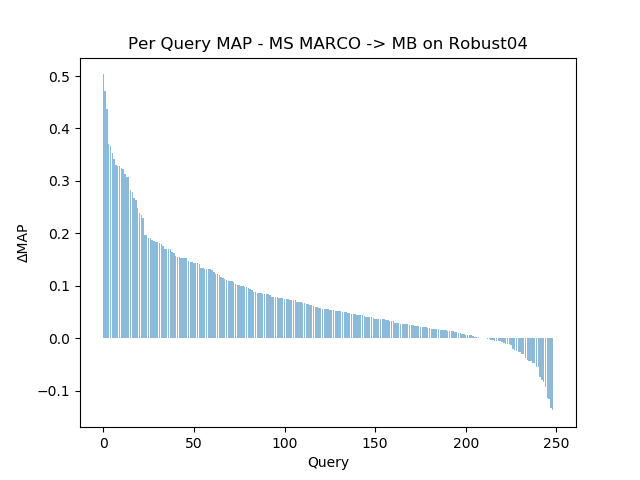
\includegraphics[width=\textwidth]{perquery1.png}
    \end{minipage}\hfill
    \begin{minipage}{0.3\textwidth}
        \centering
        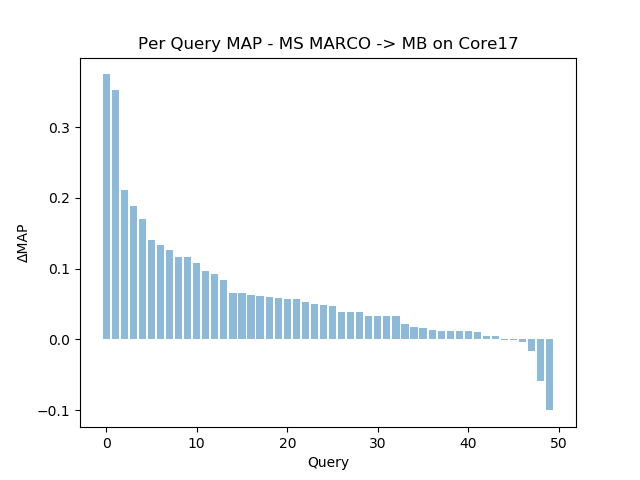
\includegraphics[width=\textwidth]{perquery2.png}
    \end{minipage}\hfill
    \begin{minipage}{0.3\textwidth}
        \centering
        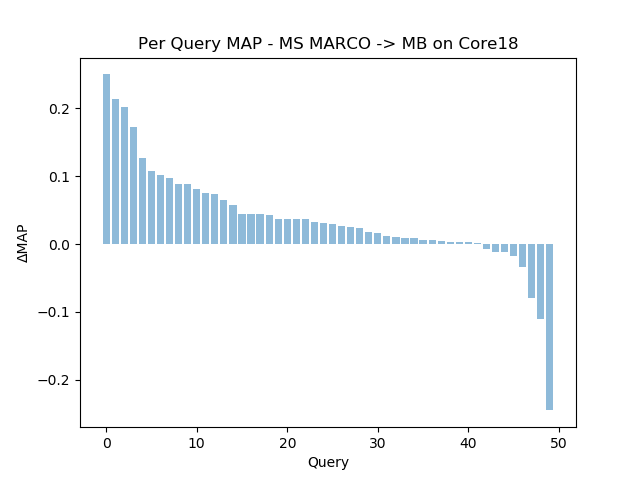
\includegraphics[width=\textwidth]{perquery3.png}
    \end{minipage}
\caption{Per-query difference in AP between $ \textrm{BERT}(\textrm{MS MARCO}\rightarrow\textrm{MB}) $ and the BM25+RM3 baseline on Robust04, Core17 and Core18.}
\label{fig:perquery-msmarcomb}
\end{figure}

%\begin{figure}[b!]
%	\centering
%    \begin{minipage}{0.3\textwidth}
%        \centering
%        \includegraphics[width=\textwidth]{perquery4.png} % first figure itself
%    \end{minipage}\hfill
%    \begin{minipage}{0.3\textwidth}
%        \centering
%        \includegraphics[width=\textwidth]{perquery5.png} % second figure itself
%    \end{minipage}\hfill
%    \begin{minipage}{0.3\textwidth}
%        \centering
%        \includegraphics[width=\textwidth]{perquery6.png} % second figure itself
%    \end{minipage}
%\caption{Per-query difference in AP between $ \textrm{BERT}(\textrm{CAR}) $ and the BM25+RM3 baseline on Robust04, Core17 and Core18.}
%\label{fig:perquery-car}
%\end{figure}

Our results in Table \ref{tab:results-robust04} serve as an overview of the effect of training data on cross-domain relevance transfer.
However, they do not reveal much with respect to the particular strengths and weaknesses of each model compared to the baseline.
To gain further insight into the characteristics of our models, we analyze the per-query retrieval effectiveness of each model compared to the baseline on Robust04, Core17 and Core18.

Figure \ref{fig:perquery-msmarcomb} plot the $\Delta$ AP per query between our best model, $ \textrm{BERT}(\textrm{MS MARCO}\rightarrow\textrm{MB}) $, and the baseline sorted in descending order.
$ \textrm{BERT}(\textrm{MS MARCO}\rightarrow\textrm{MB}) $ performs better than the baseline for 83\%, 88\% and 84\% of the queries on Robust04, Core17 and Core18 respectively, highlighting the usefulness of relevance signals learned from MS MARCO and MB with BERT.
One of the best performing queries across all three collections is \texttt{human stampede} while one of the worst is \texttt{flavr savr tomato}.
Manual inspection of top scoring sentences for \texttt{flavr savr tomato} show that our model matches terms semantically close to ``tomato'' but not relevant to the query phrase itself while the BM25+RM3 baseline looks for direct query matches, therefore ranking documents correctly.

%Repeating the same analysis for our worst model $ \textrm{BERT}(\textrm{CAR}) $, we present the results in Figure \ref{fig:perquery-car}.
%This model outperforms the baseline in 57\%, 80\% and 34\% of the Robust04, Core17 and Core18 queries respectively.
%Not only does this model perform less accurately for much fewer queries, but it is also less stable than $ \textrm{BERT}(\textrm{MS MARCO}\rightarrow\textrm{MB}) $.
%The queries \texttt{polygamy polyandry polygyny} and \texttt{women driving in Saudi Arabia} appear to be particularly difficult for BERT based models to correctly match.

%\myworries{TODO}
%In order to compare the characteristics of the two models that cause them to either excel or fail, we look into the ranking of documents for the best and worst performing queries for both.
%Specifically, we sample sentences from relevant and non-relevant documents for the given query and compare how their rank these documents.

%\begin{table}[]
%\begin{tabular}{|c|c|c|c|c|c|}
%\hline
%\multirow{2}{*}{\textbf{Query}}                       & \multirow{2}{*}{\textbf{Document ID}} & \multirow{2}{*}{\textbf{Sentence}}                                                                                                                                                                                            & \multicolumn{3}{c|}{\textbf{Rank}}                                             \\ \cline{4-6} 
%                                                      &                                       &                                                                                                                                                                                                                               & \textbf{Baseline} & \textbf{MS MARCO + MB} & \multicolumn{1}{l|}{\textbf{CAR}} \\ \hline
%\multirow{2}{*}{\textbf{372: native american casino}} & LA061290-0112                         & The Sycuan Reservation, one of 18 American Indian reservations in Southern California, operates a gaming center offering high-stakes bingo and poker seven days a week, bringing in more than \$20 million in revenues a year & 223               & 9                      & 197                               \\ \cline{2-6} 
%                                                      & FT941-13912                           & Yet, gambling on its own is not enough as Atlantic City, on the east coast in New Jersey, has discovered - to its cost.                                                                                                       & 12                & 38                     & 9                                 \\ \hline
%\end{tabular}
%\end{table}

\section{Effect of Length}

\subsection{Query Length}

\begin{table*}[b!]
\centering\resizebox{0.7\columnwidth}{!}{
\begin{tabular}{lcc ccccc}
\toprule
 & \multicolumn{5}{c}{\textbf{Query Length}} \\
 \cmidrule(lr){2-6}
{\bf Model} & {\bf 1} & {\bf 2} & {\bf 3}   & {\bf 4}  & {\bf 5} \\
\toprule
\textbf{BM25+RM3} & 0.3889 & 0.2975 & 0.2760 & 0.3089 & 0.2972 \\
\midrule
\textbf{$ \textrm{BERT}(\textrm{MB}) $} & 0.4145 & 0.3624 & 0.3230 & 0.3681 & 0.4172 \\
\midrule
\textbf{$ \textrm{BERT}(\textrm{CAR}) $} & 0.3978 & 0.3112 & 0.2871 & 0.3288 & 0.2844 \\
\midrule
\textbf{$ \textrm{BERT}(\textrm{MS MARCO}) $} & 0.3997 & 0.3117 & 0.2872 & 0.3289 & 0.2871 \\
\midrule
\textbf{$ \textrm{BERT}(\textrm{CAR}\rightarrow\textrm{MB}) $} & 0.4202 & 0.3603 & 0.3296 & 0.3757 & 0.4926  \\
\midrule
\textbf{$ \textrm{BERT}(\textrm{MS MARCO}\rightarrow\textrm{MB}) $} & 0.4253 & 0.3885 & 0.3480 & 0.4077 & 0.5627 \\
\bottomrule
\end{tabular}
}
\caption{Average AP with respect to query length on Robust04.}
\label{tab:results-query-length}
\end{table*}

To investigate the ability of BERT to exploit context-aware representations of the queries, we study the trend of effectiveness across increasing query lengths on Robust04.
We conjecture that longer queries would give our models richer context to work with, therefore increasing retrieval effectiveness.
To this end, we categorize the 250 queries from the Robust Track by the number of tokens, and calculate the average AP per query length, i.e: from 1 to 5.
The majority of the queries (56\%) are composed of three tokens, and only a small fraction (5\%) have either only a single token or five tokens.
This approach is somewhat limited by the narrow range of query lengths, but still gives insight into the effect of query length on each model's effectiveness.

The average AP per query length for each model is shown in Table \ref{tab:results-query-length}.
We only report the best results for each model considering any number of top sentences.
The average AP for the BM25+RM3 baseline drops by 24\% from a single token query to a query with five tokens, indicating that exact term-matching is more effective for fewer number of terms.
Furthermore, the improvements introduced by our models follow a similar pattern to when they are evaluated over all queries as shown in Table \ref{tab:results}, with $ \textrm{BERT}(\textrm{MS MARCO}\rightarrow\textrm{MB}) $ being the best model across all query lengths.
Similar to the baseline, $ \textrm{BERT}(\textrm{CAR}) $ and $ \textrm{BERT}(\textrm{MS MARCO}) $ experience a gradual decline in AP as the query length increases from 1 to 5, leading to an overall 29\% and 28\% decrease respectively.
Note, however, that the decrease in AP is not continuous at each step but reaches a minimum at query length 3 and a maximum at query length 4.

More interestingly, while increasing query length results in a decrease in AP across all the other models, $ \textrm{BERT}(\textrm{MB}) $, $ \textrm{BERT}(\textrm{CAR}\rightarrow\textrm{MB}) $ and $ \textrm{BERT}(\textrm{MS MARCO}\rightarrow\textrm{MB}) $ in fact perform better at query length 5 than at 1.
However, due to the fairly small sample size for query length 5 it is not possible to draw generalizable conclusions from this observation.
Nevertheless, the effectiveness of the best model  $ \textrm{BERT}(\textrm{MS MARCO}\rightarrow\textrm{MB}) $ degrades much less where the minimum usually occurs, i.e: query length 3, compared to the baseline, $ \textrm{BERT}(\textrm{CAR}) $ and $ \textrm{BERT}(\textrm{MS MARCO}) $, showing that they are indeed able to use contextualized query representations most effectively.
%It might be helpful to manually inspect rankings for each query length or to use a different averaging technique less sensitive to sample size in order to better reason about this observation; however, we leave this for future work.

\subsection{Document Length}

\begin{table*}[t!]
\centering\resizebox{0.7\columnwidth}{!}{
\begin{tabular}{lcc ccc}
\toprule
 & \multicolumn{3}{c}{\textbf{Robust04}} \\
 \cmidrule(lr){2-4}
{\bf Model} & {\bf AP} & {\bf P@20} & {\bf NDCG@20}  \\
\toprule
\textbf{$ \textrm{BERT}(\textrm{CAR}^{\star}) $} & 0.3030 & 0.3980 & 0.4520 \\
\midrule
\textbf{$ \textrm{BERT}(\textrm{MS MARCO}^{\star}) $} & 0.3300 & 0.4309 & 0.4906 \\
\bottomrule
\end{tabular}
}
\caption{Ranking effectiveness on shortened MS MARCO and CAR evaluated on Robust04.}
\label{tab:results-chopped}
\end{table*}

%Add also for Core*!
It is interesting to note that fine-tuning on MS MARCO or CAR alone results in marginal improvements over the baseline, if any, as shown in the second and third blocks of Table \ref{tab:results}.
Considering any number of top scoring sentences, $ \textrm{BERT}(\textrm{CAR}) $ and $ \textrm{BERT}(\textrm{MS MARCO}) $ both outperform the BM25+RM3 baseline by 1.2 AP on Robust04 with similar gains in P@20 and NDCG@20.
Although still statistically significant, these improvements are much lower than those gained with fine-tuning on MB (5 AP).
Moreover, both models in fact perform worse than the baseline on both Core17 and Core18.

We attribute this observation to the length mismatch between the training and evaluation text lengths.
After splitting documents into chunks that fit the maximum input that BERT can handle, the average number of tokens in Robust04, Core17 and Core17 sentences is 19, which is fairly close to the the average number of tokens in tweets (15).
However, MS MARCO and CAR passages are much longer.
It is possible that the difference in document length may be causing issues with relevance transfer across domains.

To validate this hypothesis, we divide MS MARCO and CAR passages into chunks the same size as Robust04 sentences, and train BERT for relevance prediction.
The ranking effectiveness of $ \textrm{BERT}(\textrm{CAR}^{\star}) $ and $ \textrm{BERT}(\textrm{MS MARCO}^{\star}) $ trained on the shortened data is shown in Table \ref{tab:results-chopped}.
For $ \textrm{BERT}(\textrm{CAR}^{\star}) $, AP only increases by 0.5 upon fine-tuning on the shortened data, and is still not comparable to $ \textrm{BERT}(\textrm{MB}) $.
However, the change in document length results in an increase of almost 3 AP for $ \textrm{BERT}(\textrm{MS MARCO}^{\star}) $, thus approaching $ \textrm{BERT}(\textrm{MB}) $ in all metrics.
From this finding we infer that while comparable document length is an important consideration for cross-domain relevance transfer, there may be other factors at play that need to be investigated.
%\myworries{Future work...}

%\subsection{Matching Tendencies}

\section{Semantic Matching}

\begin{table*}[t!]
\centering\resizebox{0.7\columnwidth}{!}{
\begin{tabular}{lcc ccc}
\toprule
 & \multicolumn{3}{c}{\textbf{Pruned Robust04}} \\
 \cmidrule(lr){2-4}
{\bf Model} & {\bf AP} & {\bf P@20} & {\bf NDCG@20}  \\
\toprule
\textbf{BM25+RM3} & 0.2903 & 0.3821 & 0.4407 \\
\midrule
\textbf{$ \textrm{BERT} (\textrm{MB}) $} & 0.3031 & 0.4014 & 0.4580 \\
\midrule
\textbf{$ \textrm{BERT} (\textrm{CAR}) $} & 0.2959 & 0.3936 & 0.4480 \\
\midrule
\textbf{$ \textrm{BERT} (\textrm{MS MARCO}) $} & 0.2962 & 0.3936 & 0.4483 \\
\midrule
\textbf{$ \textrm{BERT} (\textrm{CAR}\rightarrow\textrm{MB}) $} & 0.3037 & 0.3998 & 0.4527 \\
\midrule
\textbf{$ \textrm{BERT} (\textrm{MS MARCO}\rightarrow\textrm{MB}) $} & 0.3101 & 0.4102 & 0.4639 \\
\bottomrule
\end{tabular}
}
\caption{Retrieval effectiveness on pruned Robust04.}
\label{tab:results-pruned}
\end{table*}

\begin{figure}
	\centering
    \begin{minipage}{0.3\textwidth}
        \centering
        \includegraphics[width=\textwidth]{vis1.png}
    \end{minipage}\hfill
    \begin{minipage}{0.3\textwidth}
        \centering
        \includegraphics[width=\textwidth]{vis2.png}
    \end{minipage}\hfill
    \begin{minipage}{0.3\textwidth}
        \centering
        \includegraphics[width=\textwidth]{vis3.png}
    \end{minipage}
     \begin{minipage}{0.3\textwidth}
        \centering
        \includegraphics[width=\textwidth]{vis4.png}
    \end{minipage}\hfill
    \begin{minipage}{0.3\textwidth}
        \centering
        \includegraphics[width=\textwidth]{vis5.png}
    \end{minipage}\hfill
    \begin{minipage}{0.3\textwidth}
        \centering
        \includegraphics[width=\textwidth]{vis6.png}
    \end{minipage}
\caption{Attention visualizations of $ \textrm{BERT} (\textrm{MS MARCO}\rightarrow\textrm{MB}) $ for a sentence with a high BERT score for the query \texttt{international art crime}.}
\label{fig:attention}
\end{figure}

To isolate the contribution of BERT, we filter sentences in Robust04 that don't contain any of the query terms.
This essentially eliminates the impact of exact matching on the sentence relevance scores, allowing us to verify whether BERT successfully leverages semantic cues in the documents.
Table \ref{tab:results-pruned} displays the retrieval effectiveness of all models on the ``pruned'' Robust04 dataset.
Similar to Table \ref{tab:results-query-length} we only report the best results for each model.

As expected, filtering Robust04 sentences leads to a decrease in all metrics across all models, which indicates that exact matching signals are still valuable in relevance predictions over long documents.
However, notice that the all models still perform better than the baseline; in other words, they indeed successfully perform semantic matching with notable gains.
The improvements over the baseline follow the same trend as the results in Table \ref{tab:results} for all models.
While $ \textrm{BERT} (\textrm{CAR}) $ and $ \textrm{BERT} (\textrm{MS MARCO}) $ yield minor improvements over the baseline when sentences that contain exact query matches are removed, the best performing model $ \textrm{BERT} (\textrm{MS MARCO}\rightarrow\textrm{MB}) $ still significantly outperforms the baseline.
Furthermore, the drop in AP caused by filtering sentences is also the highest for the best performing model, indicating that this model is able to exploit both exact and semantic matching signals.
The overall effectiveness of this model on the original Robust04 dataset may be owing to the joint relevance matching power demonstrated in this experiment.

To further investigate the semantic matching power of BERT, we visualize the attention of our models at different layers.
Having been pretrained on massive amounts of data for language modeling, we expect BERT to capture various semantic relationships helpful for relevance prediction.
Figure \ref{fig:attention} visualizes the attention of our best model $ \textrm{BERT} (\textrm{MS MARCO}\rightarrow\textrm{MB}) $ for one of the top scoring sentences for the query 322 \texttt{international art crime}.
Note that the sentence does not contain any exact matches with the query terms and is nonetheless relevant to the query.
The top three images illustrate the attention for the query term ``art'' at increasingly deeper layers (0, 6 and 9) and the bottom three for the query term ``crime''.
We see that the model attends to related terms such as ``renaissance'' and ``paintings'' for the term ``art'', and ``robbers'' for crime, therefore giving this particular sentence a high relevance score.
On the other hand, these terms are not recognized by term-matching techniques like BM25 as relevant.
This highlights how the semantic knowledge captured by BERT directly help with relevance modeling on newswire articles.

%\subsubsection{Exact Matching}

%\begin{table*}[b!]
%\centering\resizebox{0.7\columnwidth}{!}{
%\begin{tabular}{lll lllll}
%\toprule
% & \multicolumn{5}{c}{\textbf{Fraction of Query Term}} \\
% \cmidrule(lr){2-6}
%{\bf Model} & {\bf [0.0, 0.01)} & {\bf [0.01, 0.02)} & {\bf [0.02, 0.03)} \\
%\toprule
%BM25+RM3 &  \\
%\midrule
%$ \textrm{BERT}(\textrm{MB}) $ &  \\
%\midrule
%$ \textrm{BERT}(\textrm{CAR}) $ &  \\
%\midrule
%$ \textrm{BERT}(\textrm{MS MARCO}) $ &  \\
%\midrule
%$ \textrm{BERT}(\textrm{CAR}\rightarrow\textrm{MB}) $ &   \\
%\midrule
%$ \textrm{BERT}(\textrm{MS MARCO}\rightarrow\textrm{MB}) $ &  \\
%\bottomrule
%\end{tabular}
%}
%\caption{\myworries{TODO}}
%\label{tab:results-query-terms}
%\end{table*}

%BM25 favors documents with frequent occurrences of query terms which is not necessarily the case of our BERT-based models.
%\myworries{Hypothesis}
%Therefore, we calculate the fraction of query terms (FQT) in the top k documents for each query across all models, removing stopwords and punctuation.
%We average the FQT across all retrieved documents for each query:
%
%\begin{equation}
%FQT(q) = \frac{1}{k} \sum^k _{i=1} \frac{N(d_i, q)}{|d_i|}
%\end{equation}
%
%where $ N(d_i, q) $ denotes the number of occurrences fo query tokens $ q $ in document $ d_i $.
%\myworries{limit k to 10 to avoid noise?}
%\myworries{Divide into 3 buckets instead?}
%\myworries{FQT average for each model}
%\myworries{Comment}
%
%Because BM25 relies too much on query term frequency, it may rank documents that contain multiple repetitions of query words but do not actually convey any useful information too highly.
%Therefore, we expect the effectiveness of BM25 to drop more significantly with increasing FQT.
%To observe how retrieval effectiveness changes across different ranges of FQT, we split the values into \myworries{X} buckets and calculate the average MAP for each bucket.
%\myworries{Comment}
%\myworries{Give examples of useless high FQT}